\chapter{Risultati dei Algoritmi di Machine Learning}
\label{cap:RisML}
%**************************************************************
\intro{Questo capitolo illustrerà i risultati ottenuti dai algoritmi K-Nearest-Neighbors (K-NN),  Support Vector Machine (SVM), Decision Tree, Random Forest e in fine AdaBoost.  
}

\section{Premesse}
Si sottolinea che purtroppo, i metodi di \emph{machine learning} non consentono un'analisi interpretativa dei dati come i metodi di \emph{data mining}. Per questo verranno presentati solo i risultati delle predizioni con le relative metriche.\\
Durante la fase di \emph{preprocessing} i dati sono stati standardizzati attraverso la funzione \textsf{StandardScaler()} del linguaggio Python, ovvero tutti i dati per ogni \emph{feature} sono stati centrati per ottenere varianza 1 e media 0. Questa operazione è stata eseguita per poter rendere le \emph{features} comparabile tra loro. Come già verificato nel Capitolo \ref{cap:Analisi} non ci sono valori mancati. Durante la fase di \emph{feature selection} si è scelto di utilizzare le \emph{features} che erano state utilizzate per il modello Bradley-Terry escludendo ancora il numero di gol fatti dalla squadra di casa e dagli ospiti. Questo perché durante una prima fase iniziale di verifica degli algoritmi, il Decision Tree e la Random Forest grazie a queste \emph{feature} ottenevano un’accuratezza pari a 1. Questo fenomeno è spiegabile dal fatto che sapere il numero di gol segnati in una partita indica implicitamente l'esito della partita stessa. Quindi per non rendere inutili le altre \emph{feature}, il numero di gol segnati dalla squadra di casa e dagli ospiti non sono stati presi in considerazione. Ciononostante, si sottolinea la bontà dei due algoritmi che sono riusciti a trovare la correlazione precedentemente illustrata. \\
L'attività di predizione verrà condotta suddividendo il \emph{dataset} in un insieme di training (80\%) e uno di test (20\%).\\
Tutti le funzioni utilizzate per rendere utilizzabile il \emph{dataset} sono indicate nella sezione \ref{code:ml}.

\section{Ulteriori metriche}
La capacità predittiva di un modello sarà valutata con le metriche illustrate nel Capitolo \ref{cap:risultatiDM} più l'impiego di ulteriori metriche, ovvero:
\begin{itemize}
	\item \textsf{Precision}. Misura il grado di correttezza del sistema. Indica il rapporto tra il numero di predizioni identificate correttamente con la categoria \emph{k} e il numero totale delle osservazione classificate con la categoria \emph{k} $\in \{1,..K\}$.
	\item \textsf{Area Under the Curve}. La Area Under the Curve (AUC) rappresenta l'area al di sotto della curva ROC, che è una rappresentazione grafica del rapporto tra specificità e sensibilità.
	L'AUC è una metrica che va da 0 a 1, dove un valore più alto indica una migliore prestazione di classificazione. L'AUC permette di confrontare le performance di classificatori diversi, poiché è indipendente dalla soglia di classificazione e fornisce un riassunto delle prestazioni del classificatore.
\end{itemize}

\section{K-Nearest-Neighbors}
L'algoritmo K-Nearest-Neighbors è risultato essere semplice da applicare ottenendo complessivamente discreti risultati in fase di predizione. Per scegliere i valori migliori per gli iperparametri si è applicato la K-Fold Cross Validation con \emph{k = 10}.\\
Gli iperparametri valutati sono stati i seguenti:
\begin{itemize}
	\item \textsf{n\_neighbors}. Indica il numero di vicini. Si sono verificati i valori da tre fino a 163 vicini, con un aumento unitario di 1.
	\item \textsf{p} indica il parametro potenza della distanza di Minkowski. Si sono verificati i valori \emph{p=1} (Manhattan distance) e \emph{p=2} (Euclidean distance).
\end{itemize}

Nella Figura \ref{fig:knnCV} viene mostrato l'andamento della Cross Validation per ogni valore dei iperparametri.
\begin{figure}[h]
	\begin{center}
		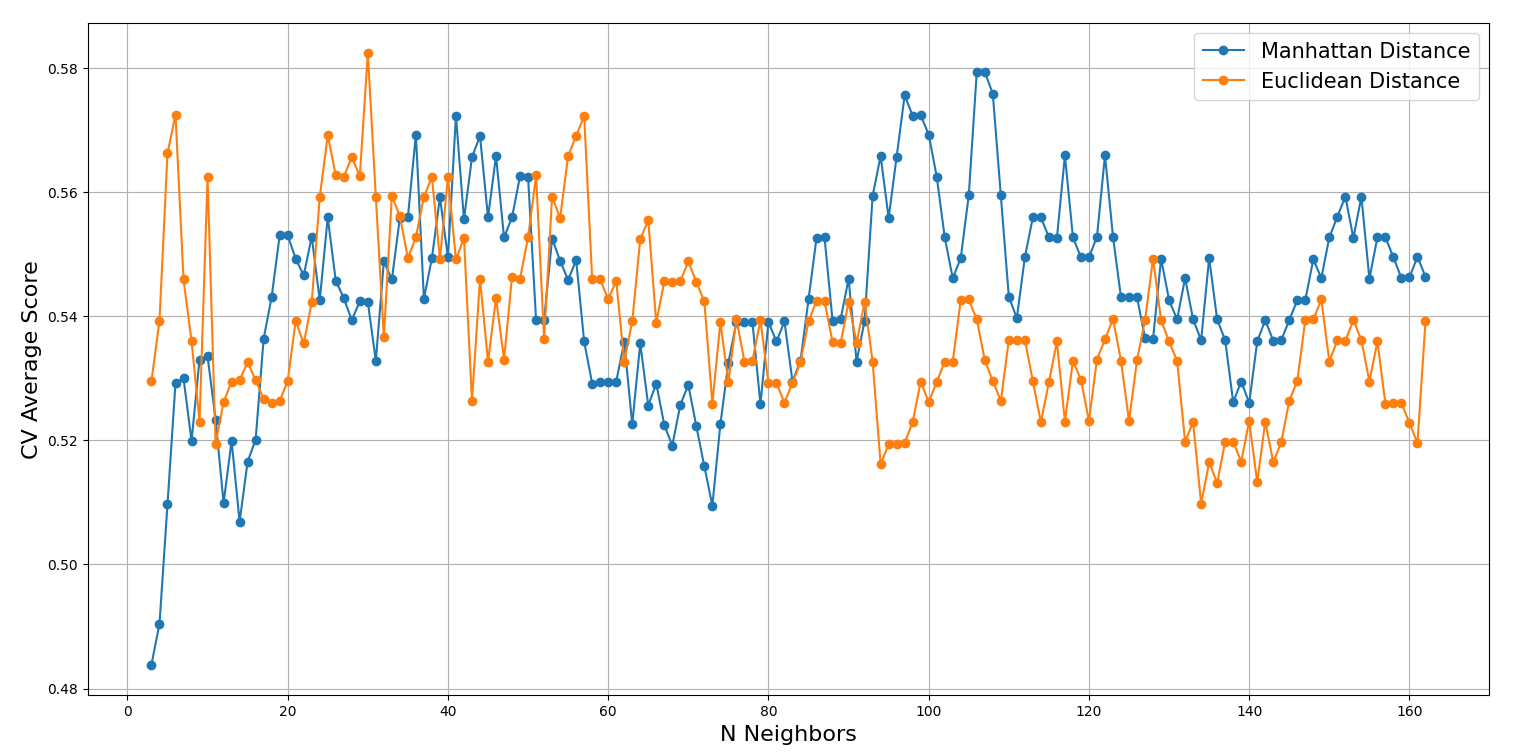
\includegraphics[scale=0.35]{knnCV.png}
		\caption{Grafico dell'andamento della media dell'accuratezza per ogni valore dell'iperparametro N Neighbors e per ogni tipo di metrica di distanza utilizzata durante l'applicazione della Cross Validation con 10 fold per il modello K-Nearest-Neighbors. Ogni punto è un classificatore con un certo numero di vicini. La linea blu indica l'andamento con la distanza di Manhattan mentre la linea arancione l'andamento con la distanza euclidea.
		} 
		\label{fig:knnCV}
	\end{center}
\end{figure}

Quello che si può notare dalla figura è che inizialmente con pochi vicini la distanza euclidea risulta essere migliore nella fase di training nel \emph{validation} \emph{set} ma con l'aumentare del numero dei vicini la distanza di Manhattan ottiene risultati migliori. \\
Secondo la Cross Validation i parametri migliori sono stati: il valore 30 come numero di vicini e la distanza euclidea come metrica della distanza da utilizzare. L'accuratezza ottenuta nel \emph{validation} \emph{set} è stata di 0.582.\\
Nella fase di predizione si sono ottenute le predizioni mostrate nella Figura \ref{fig:knnpre} con le relative metriche presentate nella Figura \ref{fig:knnmetrics}

\begin{figure}[h]
	\begin{center}
		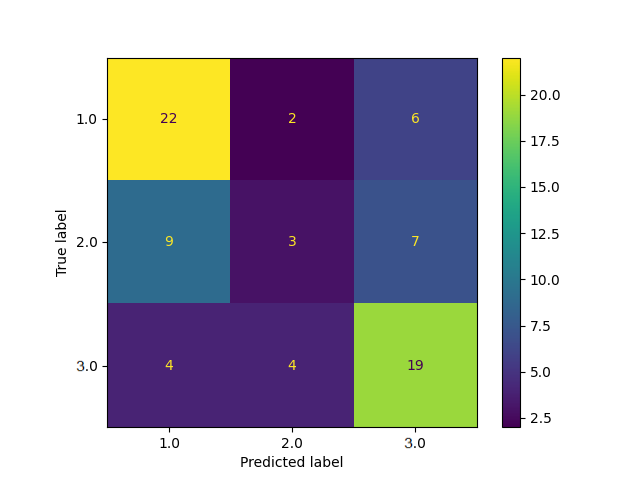
\includegraphics[scale=0.60]{tabknn.png}
		\caption{Tabella di confusione del modello K-Nearest-Neighbors con n\_neighbors = 30 e p = 2. La classe 0.0 indica la vittoria della squadra in casa, la classe 1.0 indica il pareggio tra le due squadre, la classe 2.0 indica la vittoria della squadra ospite.
		} 
		\label{fig:knnpre}
	\end{center}
\end{figure}

\begin{figure}[h]
	\begin{center}
		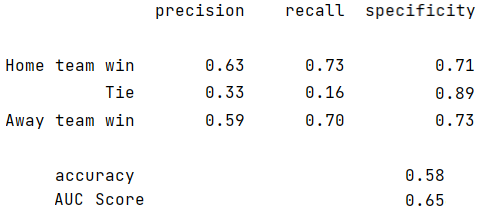
\includegraphics[scale=0.60]{metricknn.png}
		\caption{Grafico delle misurazione durante la fase di predizione del modello K-Nearest-Neighbors con n\_neighbors = 30 e p = 2.
		} 
		\label{fig:knnmetrics}
	\end{center}
\end{figure}
I risultati ottenuti sono discreti. Infatti, l'accuratezza del modello è di 0.58. Il modello ha molta difficoltà a riconoscere quando un’osservazione è di classe pareggio dato che la sensibilità è pari 0.16 ovvero delle 19 osservazioni effettivamente di classe pareggio solo tre vengono riconosciute come tali. Purtroppo, quando le osservazioni vengono etichettate con il pareggio, molto spesso viene commesso un errore di classificazione, dato che la precisione è pari a 0.33 ovvero, solo tre osservazioni su nove che sono state etichettate con la classe pareggio sono effettivamente di classe pareggio. Il modello commettendo relativamente un numero di errori basso, perché poche volte il modello etichetta con la classe pareggio ha una specificità molto alta ovvero, pari a 0.89. Risultati discreti si ottengono per la classe vittoria della squadra in casa e vittoria della squadra ospite. La precisione della classe vittoria della squadra in casa è pari a 0.63 dato che vengono etichettate erroneamente 13 osservazioni con la classe vittoria della squadra in casa. La specificità risulta pari a 0.71 mentre la sensibilità della classe vittoria della squadra in casa è pari a 0.73 ovvero, otto osservazioni su trenta non sono state identificate di classe vittoria della squadra in casa. La precisione della classe vittoria della squadra ospite è pari 0.59 poiché sono stati commessi tanti errori di classificazione. Infatti, 13 osservazioni su 32 sono state etichettate erroneamente con la classe vittoria della squadra ospite. Invece la sensibilità registrata per la classe vittoria della squadra ospite è pari a 0.70 dato che solo otto osservazioni non sono state riconosciute appartenenti alla classe vittoria della squadra ospite. Analogamente anche la specificità della classe vittoria della squadra ospite e buona dato che è pari a 0.73. Perciò il modello riesce ad individuare quasi tutte le osservazioni di classe vittoria della squadra in casa o di classe vittoria della squadra ospite, anche se per entrambe le due classi ha una discreta precisione perché molte istanze di classe pareggio vengono etichettate o con la classe vittoria della squadra in casa o con la classe vittoria della squadra ospite, abbassando così i valori della precisione delle due classi.\\
Risulta perciò non particolarmente adatto l'algoritmo K-Nearest-Neighbors per quest'analisi a causa della grande diversità tra partita e partita. Ciononostante, si ottengono discreti risultati tenendo conto del fatto delle poche osservazioni messe disposizione, ovvero 380 partite.
\section{Support Vector Machine}
L'algoritmo Support Vector Machine ha ottenuto dei buoni risultati durante la fase di predizione. Analogamente all'K-Nearest-Neighbors si è applicato la K-Fold Cross Validation con \emph{k = 10} per individuare i valori migliori per gli iperparametri.\\
Gli iperparametri valutati sono stati i seguenti:
\begin{itemize}
	\item \textsf{C}. Indica la forza applicata della penalità L2. Si sono verificati valori che vanno da 0.1 a 1.5 con un aumento unitario di 0.1.
	\item \textsf{kernel}. Indica quale funzione di kernel utilizzare. Si sono verificati i valori kernel = linear ovvero il linear kernel, kernel = rbf ovvero Gaussian Radial Basis kernel (RBF) e kernel = poly ovvero il polynomial kernel.
\end{itemize}

Nella Figura \ref{fig:svcCV} viene mostrato l'andamento della Cross Validation per ogni valore dei iperparametri.
\begin{figure}[]
	\begin{center}
		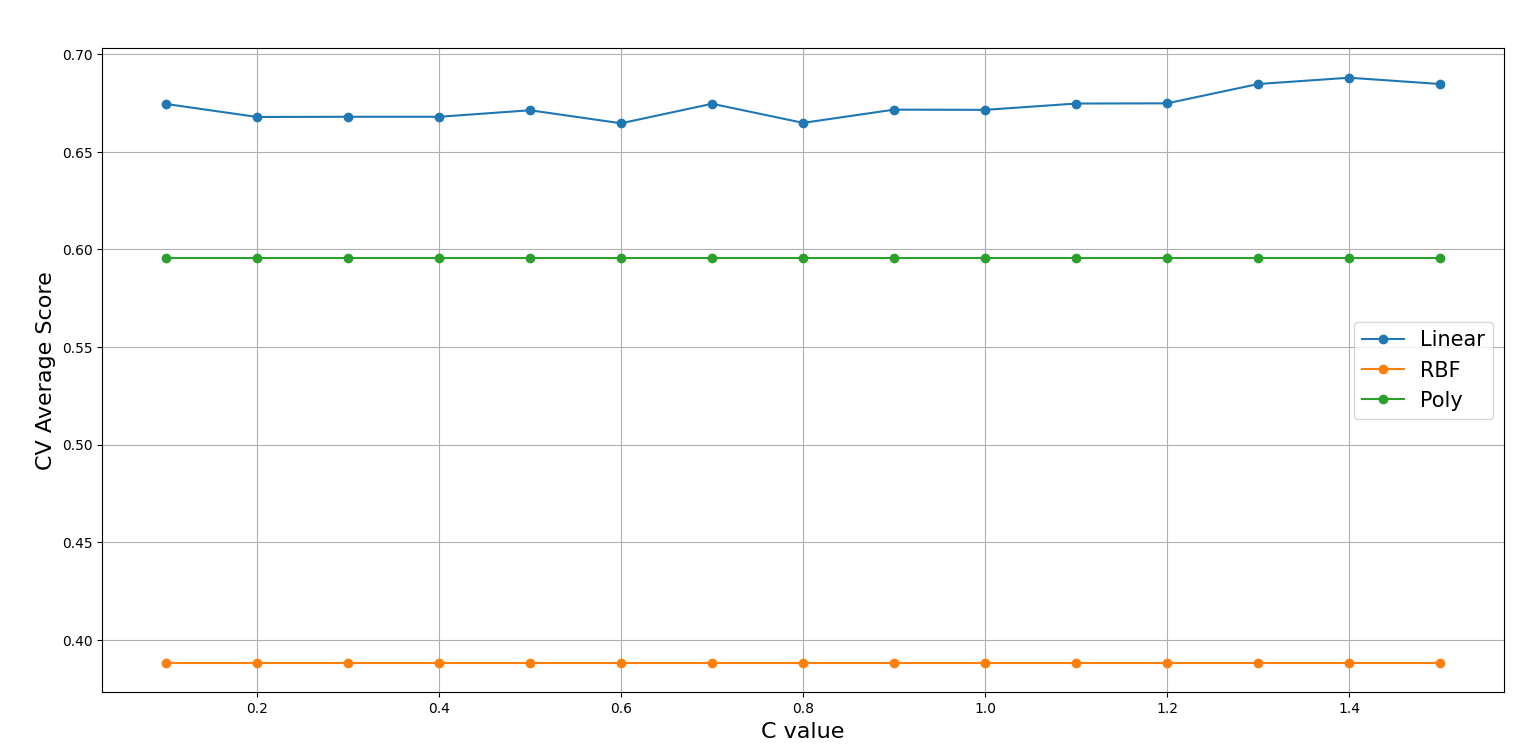
\includegraphics[scale=0.35]{svcCV.png}
		\caption{Grafico dell'andamento della media dell'accuratezza per ogni valore dell'iperparametro C e per ogni funzione kernel utilizzata durante l'applicazione della Cross Validation con 10 fold per il modello Support Vector Machine. Ogni punto è un classificatore con un certo valore di C. La linea blu indica l'andamento con la funzione linear kernel mentre la linea verde l'andamento con la funzione RBF e	la linea arancione l'andamento con la funzione polynomial kernel.
		} 
		\label{fig:svcCV}
	\end{center}
\end{figure}

Dal grafico si nota che dal punto di vista dell'accuratezza registrata nel \emph{validation} \emph{set}, il kernel tipo lineare ottiene le prestazioni migliori. Infatti, vediamo che la linea blu costantemente al di sopra rispetto alle due restanti kernel a parità del valore in C. Invece, il polynomial kernel non ha buone prestazioni; infatti, si registra che la linea arancione è costantemente al di sotto delle altre due linee perché ha valori molto più bassi di accuratezza.\\
Secondo la Cross Validation i parametri migliori sono stati: il valore 1.4 per il parametro C e il Linear kernel come funzione kernel da utilizzare.
L'accuratezza ottenuta nel \emph{validation} \emph{set} è stata di 0.683.\\ Nella fase di predizione si sono ottenute le predizioni mostrate nella Figura \ref{fig:tabsvc} con le relative metriche presentate nella Figura \ref{fig:svcmetrics}.
\begin{figure}[]
	\begin{center}
		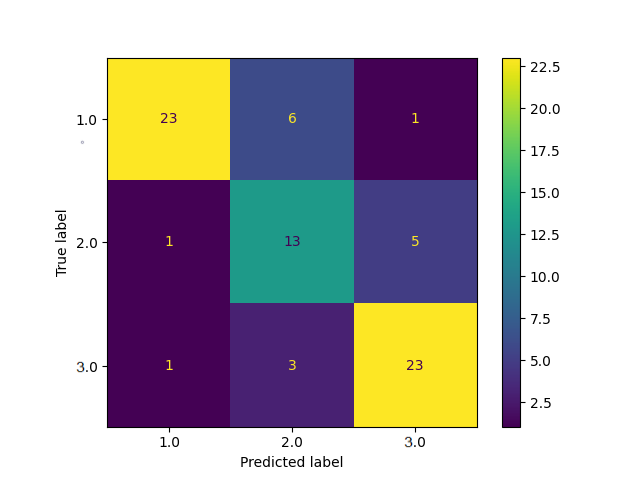
\includegraphics[scale=0.60]{tabsvc.png}
		\caption{Tabella di confusione del modello Support Vector Machine con C = 1.4 e kernel = linear. La classe 0.0 indica la vittoria della squadra in casa, la classe 1.0 indica il pareggio tra le due squadre, la classe 2.0 indica la vittoria della squadra ospite.
		} 
		\label{fig:tabsvc}
	\end{center}
\end{figure}

\begin{figure}[]
	\begin{center}
		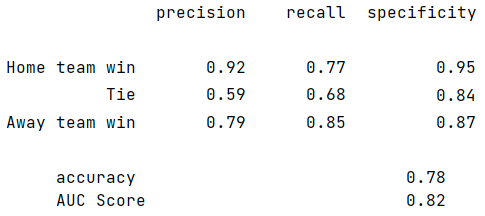
\includegraphics[scale=0.60]{metricsvc.png}
		\caption{Grafico delle misurazione durante la fase di predizione del modello Support Vector Machine con C = 1.4 e kernel = linear.
		} 
		\label{fig:svcmetrics}
	\end{center}
\end{figure}
Nonostante le poche osservazioni disponibili e l'elevato numero di \emph{features} utilizzate, i risultati ottenuti sono buoni. Infatti, l'accuratezza è di 0.78. Il modello riesce a riconoscere buona parte delle osservazioni di classe pareggio. Infatti, è stata registrata una sensibilità pari a 0.68 per la classe pareggio ovvero solo sei osservazioni di classe pareggio su 19 non sono state riconosciute come tali. Tuttavia, la precisione scende a 0.59. Infatti, nove osservazioni sono state etichettate erroneamente con la classe pareggio. Ciononostante, quest'errore non è molto grande dato che la specificità è pari a 0.84. Risultati migliori si ottengono per la classe vittoria della squadra in casa e vittoria della squadra ospite. La precisione per la classe della vittoria della squadra in casa è pari a 0.92, dato che tutte le classificazioni fatte con questa classe si sono rivelate quasi tutte corrette. Infatti, solo due osservazioni sono state etichettate erroneamente con la classe vittoria della squadra in casa. Di conseguenza anche la specificità ha un valore molto alto ovvero pari a 0.95. Tuttavia, sette osservazioni di classe vittoria della squadra di casa non sono state identificate correttamente dato la sensibilità è pari a 0.77. Invece La sensibilità della classe vittoria della squadra ospite è pari a 0.85 dato che solo che solo quattro osservazioni non vengo identificate di classe vittoria della squadra ospite. Ciononostante, si registra una buona precisione pari a 0.79 ovvero delle 29 osservazioni classificate con la classe vittoria della squadra ospite solo sei risultano essere di un'altra classe. Buone prestazioni anche per la specificità della classe vittoria della squadra ospite che pari a 0.87.\\
Risulta perciò adatto l'algoritmo Support Vector Machine per quest'analisi nonostante la grande diversità da partita a partita e le poche osservazioni messe disposizione, ovvero 380 partite.


\section{Decision Tree}

Con l'applicazione dell'algoritmo Decision Tree sono stati registrati dei buoni risultati durante la fase di predizione. Analogamente all'K-Nearest-Neighbors si è applicato la K-Fold Cross Validation con \emph{k = 10} per individuare i valori migliori per gli iperparametri.\\
Gli iperparametri valutati sono stati i seguenti:
\begin{itemize}
	\item \textsf{max\_depth}. Indica la profondità massima dell'albero. Si sono verificati valori che vanno da 3 fino a 52, dove 52 e il numero di \emph{feature} che sono presenti nel \emph{dataset}. Inoltre, questo parametro permette di controllare l'\emph{overfitting} ovvero, se le prestazioni peggiorano durante il training, i rami più profondi dell'albero vengono tagliati.
	\item \textsf{criterion}. Indica la regola di decisione utilizzata per la creazione dell'albero. Si sono verificate le regole Gini Index e Cross Entropy.
\end{itemize}

Nella Figura \ref{fig:dtCV} viene mostrato l'andamento della Cross Validation per ogni valore dei iperparametri.
\begin{figure}[h]
	\begin{center}
		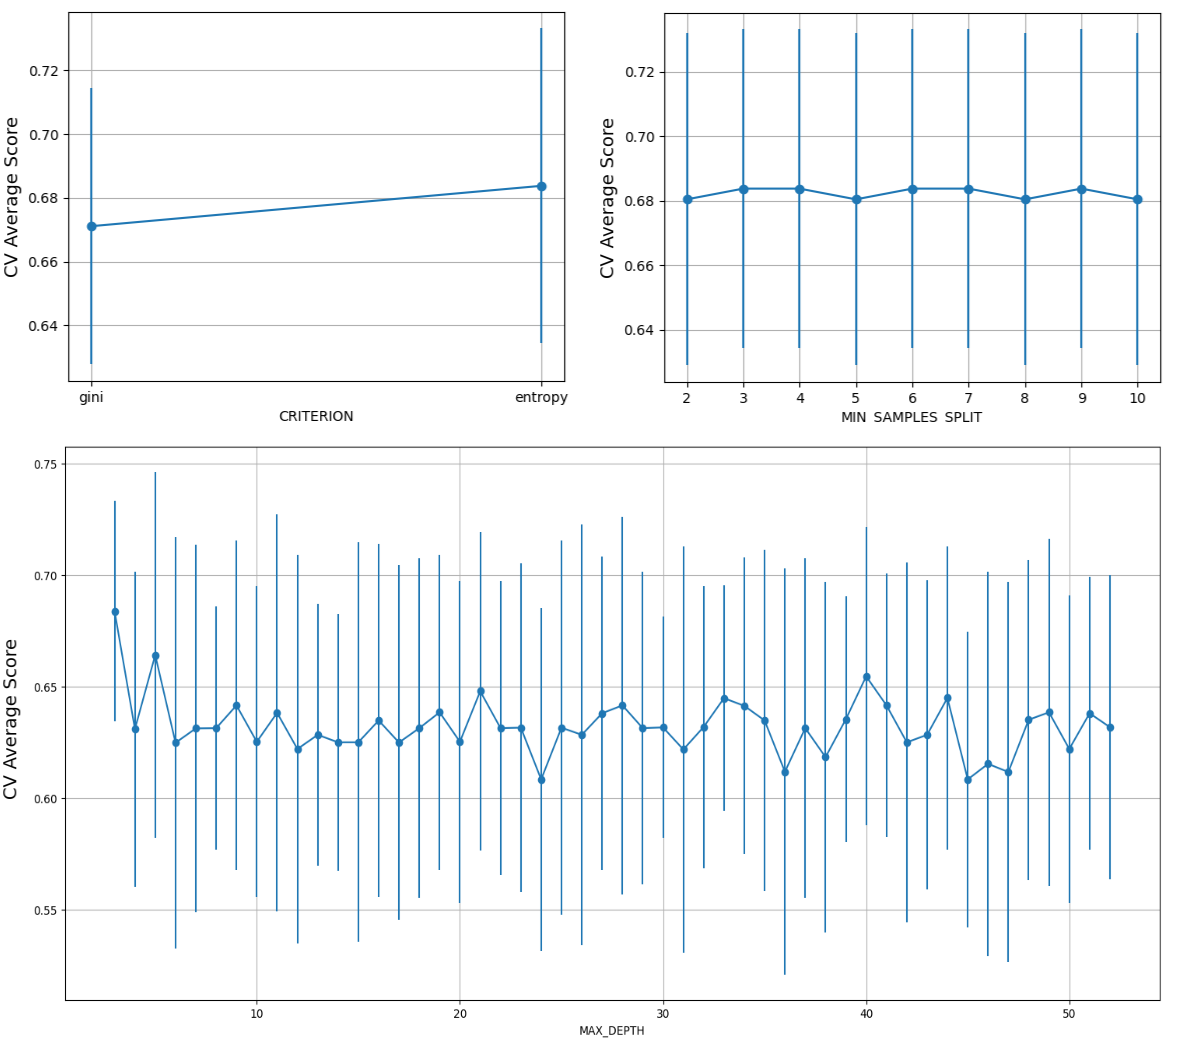
\includegraphics[scale=0.34]{dtCV.png}
		\caption{Grafico dell'andamento della media dell'accuratezza per ogni valore dell'iperparametro max\_depth e per ogni regola di decisione utilizzata durante l'applicazione della Cross Validation con 10 fold per il modello Decision Tree. Ogni punto è un classificatore con un certo limite di profondità. La linea blu indica l'andamento con la regola di decisione Gini Index mentre la linea arancione indica l'andamento con la regola di decisione Cross Entropy.
		} 
		\label{fig:dtCV}
	\end{center}
\end{figure}

Dal grafico si nota che le due regole in molte occasioni registrano un'accuratezza simile nel \emph{validation set}. Al contrario all'inizio con un numero basso di \emph{feature} la regola Cross Entropy ottiene prestazioni leggermente migliori rispetto al Gini Index. In generale vi è un'andamento irregolare. Vi è un forte decadimento delle prestazioni con l'aumento del numero di \emph{feature}, soprattutto con un numero di \emph{feature} superiore a 5.\\
Secondo la Cross Validation i parametri migliori sono stati: il valore 3 per il parametro max\_depth e la Cross Entropy come regola di decisione da utilizzare. L'accuratezza ottenuta nel \emph{validation} \emph{set} è stata di 0.684.\\
Nella fase di predizione si sono ottenute le predizioni mostrate nella Figura \ref{fig:tabdt} con le relative metriche presentate nella Figura \ref{fig:dtmetrics}.
\begin{figure}[h]
	\begin{center}
		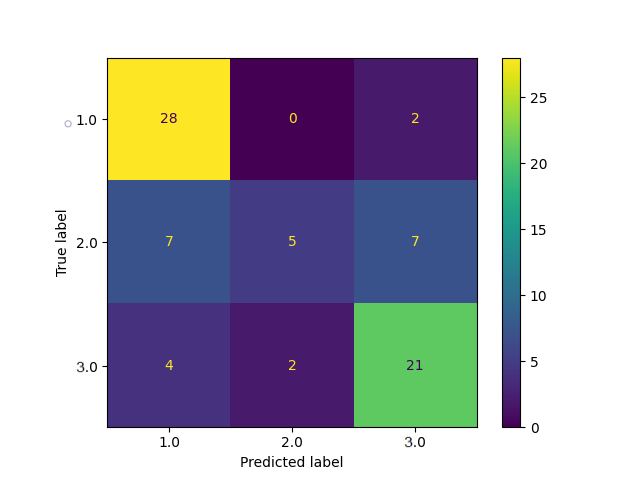
\includegraphics[scale=0.60]{tabdt.png}
		\caption{Tabella di confusione del modello Decision Tree con max\_depth = 3 e criterion = entropy. La classe 0.0 indica la vittoria della squadra in casa, la classe 1.0 indica il pareggio tra le due squadre, la classe 2.0 indica la vittoria della squadra ospite.
		} 
		\label{fig:tabdt}
	\end{center}
\end{figure}

\begin{figure}[]
	\begin{center}
		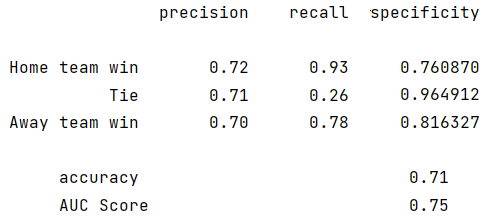
\includegraphics[scale=0.60]{metricdt.png}
		\caption{Grafico delle misurazione durante la fase di predizione del modello Decision Tree con max\_depth = 3 e criterion = entropy.
		} 
		\label{fig:dtmetrics}
	\end{center}
\end{figure}

Nonostante le poche osservazioni disponibili i risultati ottenuti sono buoni. Infatti, l'accuratezza è di 0.71. Ciononostante, il modello ha qualche difficoltà a identificare le osservazioni della classe pareggio. Infatti, si è registrata una sensibilità molto bassa pari a 0.26. Nonostante il modello etichetti un'osservazione con la classe pareggio in poche occasioni, esso sbaglia poco. Infatti ci sono solo due osservazioni etichettate erroneamente con la classe pareggio con una precisione pari a 0.71. Ovviamente la specificità nella classe pareggio è molto alta dato che il modello poche volte sbaglia ad etichettare con la classe pareggio. Buoni risultati sia per la classe vittoria della squadra di casa e sia dalla classe vittoria della squadra ospite. Infatti, per la prima classe c'è una sensibilità pari a 0.93 ovvero soltanto due osservazioni di classe vittoria della squadra in casa non sono state identificate come tali. Le prestazioni però calano nella precisione dato che undici osservazioni sono state etichettate erroneamente con la classe vittoria della squadra di casa. Di conseguenza anche la specificità è calata rispetto alla sensibilità dato che è pari a 0.76. Analogamente anche la classe vittoria della squadra ospite ha una buona sensibilità pari a 0.78, dato che sei osservazioni di classe vittoria della squadra ospite non sono state identificate come tali. Anche la precisione rimane in linea con le prestazioni della sensibilità che è pari a 0.70 ovvero, nove osservazioni sono state etichettate erroneamente con la classe vittoria della squadra ospite. Nonostante ciò, la specificità ottiene prestazioni migliori pari a 0.82.\\
Dato che l'algoritmo Decision Tree non è un algoritmo a scatola chiusa (Black box), è possibile capire quali sono state le sue scelte analizzando l'albero di decisione che ha prodotto per svolgere le sue predizioni. Nella Figura \ref{fig:dttree} viene mostrato l'albero di decisione prodotto e utilizzato durante la fase di predizione.
\begin{figure}[h]
	\begin{center}
		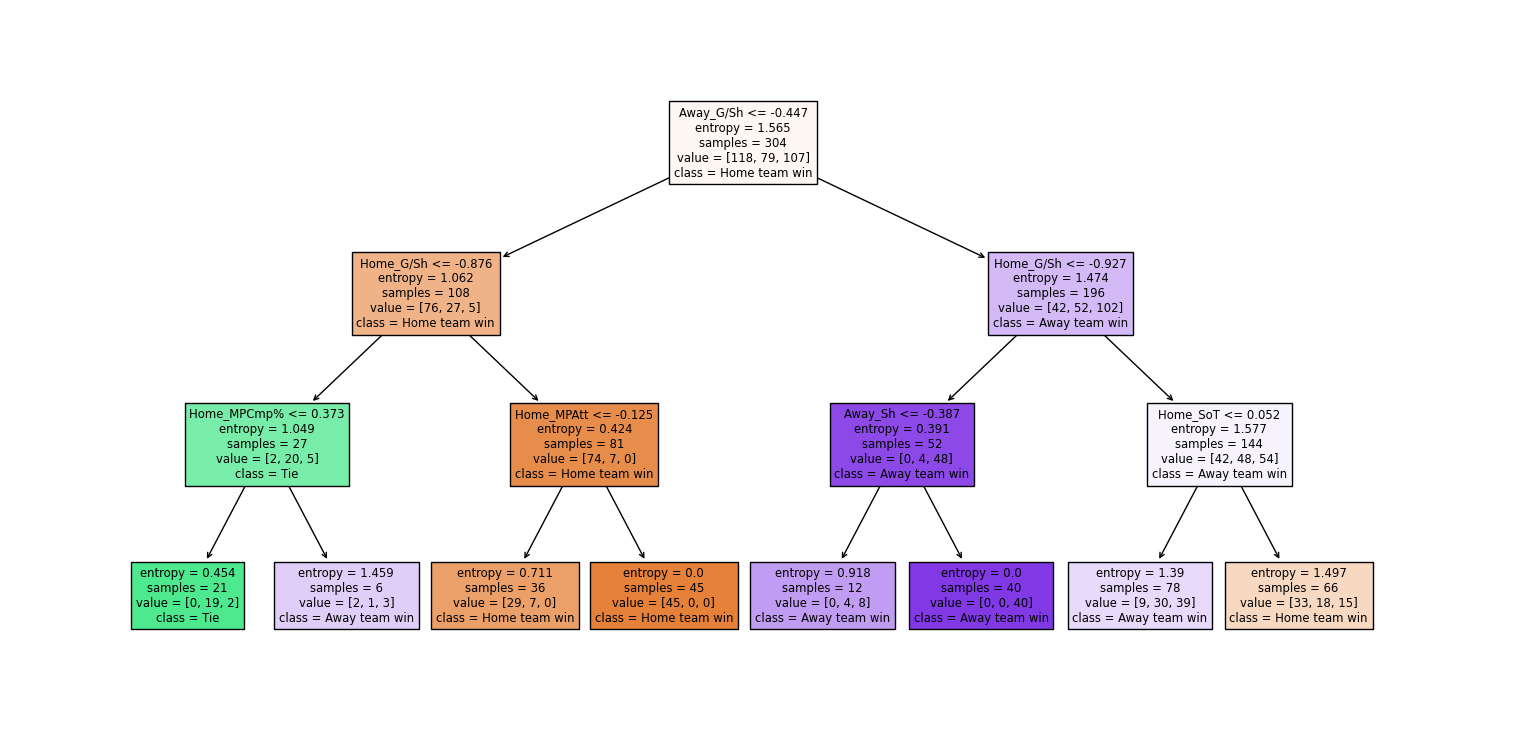
\includegraphics[height = 10cm, width = 16cm]{treedt.png}
		\caption{L'albero di decisione del modello Decision Tree con max\_depth = 3 e criterion = entropy. Per ogni nodo non foglia c'è un test che indica quale ramo scegliere asseconda del valore contenuto nell'attributo testato. Il parametro \textsf{entropy} indica l'entropia misurata. Il parametro \textsf{samples} indica il numero di istanze che soddisfano i test precedenti. Nel parametro \textsf{value} vengono riportati il numero di istanze presenti per ognuna delle tre classi. Il parametro \textsf{class} indica la classe di maggioranza nel nodo. Il colore indica la classe di maggioranza con una tonalità differente asseconda della frequenza della classe di maggioranza.
		} 
		\label{fig:dttree}
	\end{center}
\end{figure}

Perciò nell'albero mostrato in figura, per ogni nodo non foglia c'è un test che indica quale ramo scegliere asseconda del valore contenuto nell'attributo testato. Il test consiste semplicemente nel verificare se l'attributo ha un valore minore uguale o maggiore rispetto a un certo valore. Questo tipo di test permette di gestire attributi con valori continui utilizzando una soglia di decisione scelta opportunamente dell'algoritmo. Per tutti i nodi è presente il parametro \textsf{entropy} che indica l'entropia misurata. Il parametro \textsf{samples} che indica il numero di istanze che soddisfano i test precedenti. Il parametro \textsf{value} che il numero di istanze presenti per ognuna delle tre classi. Il parametro \textsf{class} che indica la classe di maggioranza nel nodo, mentre il colore indica la classe di maggioranza con una tonalità differente asseconda della frequenza della classe di maggioranza. Quando viene raggiunto un nodo foglia si classifica l'osservazione con la classe di maggioranza dato che non ci sono più attributi che permettono di distinguere le istanze.\\
Osservando l'albero, le \emph{feature} legate ai tiri si confermano di grande importanza non solo i modelli Bradley-Terry visti nel Capitolo \ref{cap:RisML} ma anche per il modello Decision Tree.\\
In conclusione, risulta essere adatto l'algoritmo Decision Tree per quest'analisi nonostante le poche osservazioni messe disposizione.

\section{Random Forest}